%%%%%%%%%%%%%%%%%%%%%%%%%%%%%%%%%%%%%%%%%%%%%%%%%%%%%%%%%%%%%%%%%%%%%%%%%%%%%%%
\documentclass[a4paper,12pt]{article}

%%%%%%%%%%%%%%%%%%%%%%%%%%%%%%%%%%%%%%%%%%%%%%%%%%%%%%%%%%%%%%%%%%%%%%%%%%%%%%%

\usepackage{extsizes}
\usepackage{cmap}
\usepackage[T2A]{fontenc}
\usepackage[utf8x]{inputenc}
\usepackage[english, russian]{babel}
\usepackage{misccorr}
\usepackage{amssymb,amsfonts,amsmath,amsthm}  % математические дополнения от АМС
\usepackage{envmath}  % многострочные формулы EqSystem
\usepackage{indentfirst} % Включение отступа первой строки раздела
\usepackage[usenames,dvipsnames]{color} % названия цветов

%%%%%%%%%%%%%%%%%%%%%%%%%%%%%%%%%%%%%%%%%%%%%%%%%%%%%%%%%%%%%%%%%%%%%%%%%%%%%%%

	% выбрать цвета:
% \definecolor{BlueGreen}{RGB}{49,152,255}

%%%%%%%%%%%%%%%%%%%%%%%%%%%%%%%%%%%%%%%%%%%%%%%%%%%%%%%%%%%%%%%%%%%%%%%%%%%%%%%

	% назначить цвета при подключении hyperref
\usepackage[unicode, colorlinks, urlcolor=magenta, linkcolor=black, pagecolor=black]{hyperref}
	% linkcolor=
	% цвет гиперссылок внутри документа, по-умолчанию red
	% pagecolor=
	% цвет гиперссылок на другие страницы внутри документа, по-умолчанию red
	% filecolor=
	% цвет гиперссылок, открывающих локальные файлы, по-умолчанию cyan
	% anchorcolor=
	% цвет текста мишени, по-умолчанию black
	% citecolor=
	% цвет библиографических ссылок, по-умолчанию green
	% urlcolor=
	% цвет гиперссылок на сетевые ресурсы, по-умолчанию magenta

%%%%%%%%%%%%%%%%%%%%%%%%%%%%%%%%%%%%%%%%%%%%%%%%%%%%%%%%%%%%%%%%%%%%%%%%%%%%%%%

	% улучшенное форматирование таблиц
\usepackage{makecell} 
\usepackage{multirow} 

%%%%%%%%%%%%%%%%%%%%%%%%%%%%%%%%%%%%%%%%%%%%%%%%%%%%%%%%%%%%%%%%%%%%%%%%%%%%%%%

	% подчеркивания
\usepackage{ulem}

%%%%%%%%%%%%%%%%%%%%%%%%%%%%%%%%%%%%%%%%%%%%%%%%%%%%%%%%%%%%%%%%%%%%%%%%%%%%%%%

	% для вставки изображений
\usepackage{graphicx} 
	%где искать изображения
\graphicspath{{img/}}

%%%%%%%%%%%%%%%%%%%%%%%%%%%%%%%%%%%%%%%%%%%%%%%%%%%%%%%%%%%%%%%%%%%%%%%%%%%%%%%
	
	% поля страницы 
\usepackage{geometry}
\geometry{left=3cm,right=2cm,top=3cm,bottom=3cm,bindingoffset=0cm}

%%%%%%%%%%%%%%%%%%%%%%%%%%%%%%%%%%%%%%%%%%%%%%%%%%%%%%%%%%%%%%%%%%%%%%%%%%%%%%%

	% Cтиль оформления chapter
% \usepackage[Glenn]{fncychap} 
	% Всего имеется семь возможных стилей: 
	% Sonny, Lenny, Glenn, Conny, Rejne, Bjarne, Bjornstrup.

%%%%%%%%%%%%%%%%%%%%%%%%%%%%%%%%%%%%%%%%%%%%%%%%%%%%%%%%%%%%%%%%%%%%%%%%%%%%%%%

	%Колинтулы страниц
\usepackage{fancyhdr} 

%%%%%%%%%%%%%%%%%%%%%%%%%%%%%%%%%%%%%%%%%%%%%%%%%%%%%%%%%%%%%%%%%%%%%%%%%%%%%%%

	% полуторный интервал
\linespread{1.3} 

	% стиль пробелов: французский - все пробелы примерно одинаковые
\frenchspacing 

	% Элементы списка второго уровня с скобочкой вместо точки
\renewcommand{\labelenumii}{\theenumii)} 

%%%%%%%%%%%%%%%%%%%%%%%%%%%%%%%%%%%%%%%%%%%%%%%%%%%%%%%%%%%%%%%%%%%%%%%%%%%%%%%  % преамбула
%%%%%%%%%%%%%%%%%%%%%%%%%%%%%%%%%%%%%%%%%%%%%%%%%%%%%%%%%%%%%%%%%%%%%%%%%%%%%%%

\newcommand{\labauthor}{Сарафанов Ф.\,Г.}
\newcommand{\labauthors}{Сарафанов Ф.\,Г.}
% \newcommand{\labauthors}{Сарафанов Ф.\,Г., Сидоров Д.\,А.}
\newcommand{\labnumber}{17}
\newcommand{\labtheme}{Осциллограф}


\newcommand{\ddt}{$\ \pm\ 0.2\ \text{с}$}
\newcommand{\ddtv}{$\ \pm\ 0.8\ \text{с}$}
\newcommand{\ddh}{$\ \pm\ 0.1\ \text{см}$}
\newcommand{\dm}{\Delta{}m}
\newcommand{\Dh}{\Delta{}x}
\newcommand{\Dl}{\Delta{}(\lambda)}
\newcommand{\dmsr}{<\Delta{}m>}
\newcommand{\el}{\varepsilon(\lambda)}

\usetikzlibrary{%
    decorations.pathreplacing,%
    decorations.pathmorphing,%
    arrows,%
    patterns
}
\newcommand{\Scale}{1}
\newcommand{\lft}{9}
\newcommand{\rft}{10.43*1.5}
\newcommand{\Xstep}{1.5}
\newcommand{\Ystep}{1.5*20}
\newcommand{\Radius}{0.1}
\newcommand{\Color}{black}
\newcommand{\Tr}{T_\text{р}}
\newcommand{\Ts}{T_\text{с}}

%%%%%%%%%%%%%%%%%%%%%%%%%%%%%%%%%%%%%%%%%%%%%%%%%%%%%%%%%%%%%%%%%%%%%%%%%%%%%%%
%%%%%%%%%%%%%%%%%%%%%%%%%%%%%%%%%%%%%%%%%%%%%%%%%%%%%%%%%%%%%%%%%%%%%%%%%%%%%%%
	%применим колонтитул к стилю страницы
\pagestyle{fancy} 
	%очистим "шапку" страницы
\fancyhead{} 
	%слева сверху на четных и справа на нечетных
\fancyhead[LE,RO]{\labauthors} 
	%справа сверху на четных и слева на нечетных
\fancyhead[LO, RE]{Отчёт по лабораторной работе №\labnumber} 
	%очистим "подвал" страницы
\fancyfoot{} 
	% номер страницы в нижнем колинтуле в центре
\fancyfoot[CO,CE]{\thepage} 

%%%%%%%%%%%%%%%%%%%%%%%%%%%%%%%%%%%%%%%%%%%%%%%%%%%%%%%%%%%%%%%%%%%%%%%%%%%%%%% % колинтулы на страницах
%%%%%%%%%%%%%%%%%%%%%%%%%%%%%%%%%%%%%%%%%%%%%%%%%%%%%%%%%%%%%%%%%%%%%%%%%%%%%%%

\usepackage{float}

\begin{document}

\begin{titlepage}

\begin{center}

{\small\textsc{Нижегородский государственный университет имени Н.\,И. Лобачевского}}
\vskip 1pt \hrule \vskip 3pt
{\small\textsc{Радиофизический факультет}}

\vfill

{\Large Отчет по лабораторной работе №\labnumber\vskip 12pt\bfseries \labtheme}
	
\end{center}

\vfill
	
\begin{flushright}
	{Выполнил студент 410 группы\\ \labauthor\vskip 12pt Принял:\\ Менсов С.\,Н.}
\end{flushright}
	
\vfill
	
\begin{center}
	Нижний Новгород, 2016
\end{center}

\end{titlepage}



\tableofcontents

\newpage
\section{Описание лабораторной установки}

\textbf{Цель работы:} ознакомление с устройством электронного осциллографа; изучение принципов работы развертки, усилителей вертикального и горизонтального каналов, получение фигур Лиссажу, изучение частотных свойств вертикального усилителя.
\vspace{1.5em}

\textbf{Оборудование:}
Осциллограф С1-1 (ЭО-7), генератор низкочастотных сигналов ГЗ-109
\vspace{1.5em}

\textbf{Приборные погрешности:} Класс точности вольтметра - 2.5, погрешности генератора: $\Delta{\nu}=2+\frac{50}{\nu}$ (20--200 Гц), $\Delta{\nu}=1+\frac{50}{\nu}$ (200 Гц--200 кГц).
\vspace{1.5em}

Электронный осциллограф — прибор, предназначенный в основном для исследования быстропротекающих процессов в электрических цепях (или не электрических процессов с помощью соответствующих преобразователей представленных в виде электрических сигналов).

В работе использован осциллограф C1-1 (ЭО-7). Его упрощенная блок-схема приведена на рисунке (рис. \ref{fig:chem})

\begin{figure}[H]
	\centering
	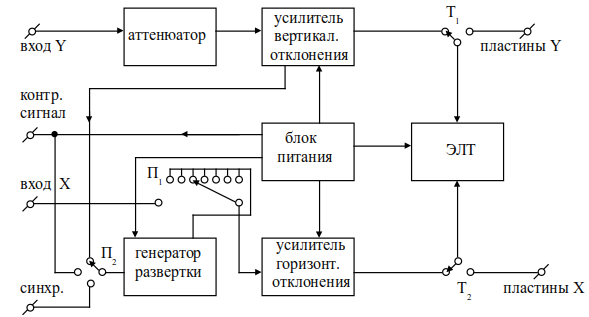
\includegraphics[width=\textwidth]{chem.png}
	\caption{Упрощенная блок-схема осциллографа}
	\label{fig:chem}
\end{figure}

Основным элементом электронного осциллографа является электронно-лучевая трубка.

\subsection{ЭЛТ осциллографа}

Электронно-лучевая трубка (рис. \ref{fig:elt}) представляет собой стеклянный баллон с тщательно откаченным воздухом с металлическими электродами.

\begin{figure}[H]
	\centering
	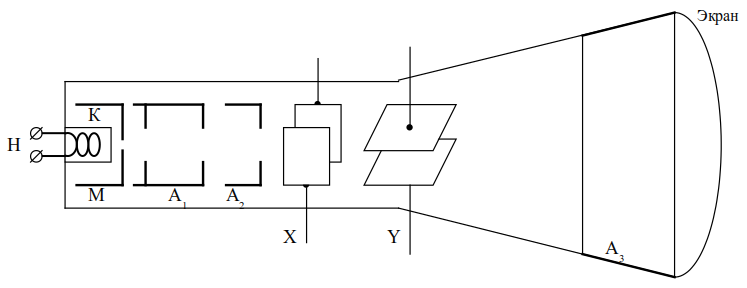
\includegraphics[width=\textwidth]{elt.png}
	\caption{Чертеж электронно-лучевой трубки осциллографа С1-1}
	\label{fig:elt}
\end{figure}

Основными частями трубки являются:
\begin{enumerate}
	\item электронная пушка
		\begin{enumerate}
			\item подогревный катод
			\item модулятор
			\item 1-й анод
			\item 2-й анод
		\end{enumerate}
	\item флуоресцирующий экран
	\item отклоняющие пластины
\end{enumerate}

Электронная пушка создает поток электронов и формирует этот поток в электронный луч.

Электронный луч, состоящий из быстро летящих электронов, направляется на флуоресцирующий экран.

Первый и второй аноды $A_1$ и $A_2$ имеют положительный потенциал относительно катода. Потенциал $A_2$ делается выше (1 -- 2 кВ), чем потенциал $A_1$ (от 100 -- 200 В). 

Конфигурация и взаимное расположение анодов подбирается таким образом, что электрическое поле, действующее на электроны, ускоряет их и собирает в тонкий луч. 

Действие электрического поля на поток электронов аналогично фокусированию светового потока оптической линзой.

Чем больше электронов в пучке, тем ярче будет пятно на экране. Величина тока в пучке регулируется напряжением на модуляторе. Фокусировка осуществляется изменением напряжения на первом аноде (изменяется конфигурация электрического поля и его фокусирующее действие).

Отклонение электронного луча производится с помощью электрических полей, создаваемых между парами взаимно-перпендикулярных отклоняющих пластин. 

Для получения на экране формы исследуемого напряжения -- осциллограммы, необходимо исследуемое напряжение подавать на вертикальные пластины, а по горизонтали заставить луч смещаться равномерно по времени, для чего на горизонтальные пластины подается пилообразное напряжение, снимаемое с генератора развертки.

Важным параметром трубки является ее чувствительность $$\varkappa=\frac{l_1l_2}{U_{A2}d}$$

\subsection{Блок развертки}

Пилообразное напряжение, с помощью которого осуществляется равномерное во времени отклонение луча в горизонтальном направлении, вырабатывается генератором развертки.

Реальный ход изменения напряжения развертки, т.е. напряжения на конденсаторе, происходит, согласно теории электрических цепей, по экспоненциальному закону. Поэтому для получения подобного пилообразному напряжения можно брать только небольшой участок экспоненты, где она несильно отличается от прямой (рис. \ref{fig:exp}).

\begin{figure}[H]
	\centering
	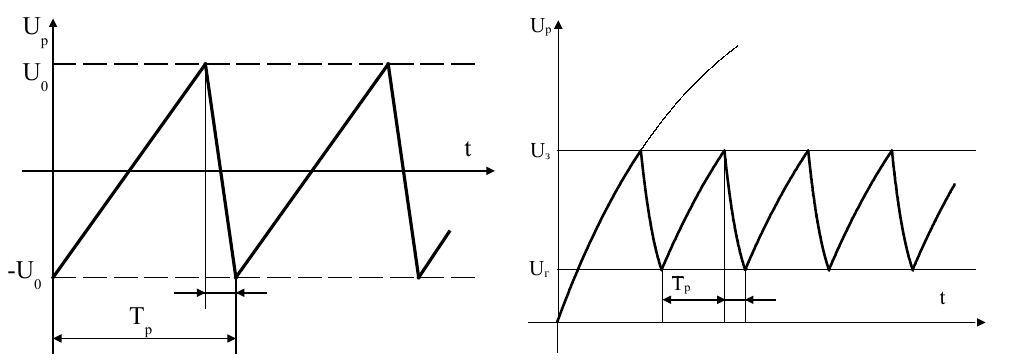
\includegraphics[width=1\textwidth]{exp.png}
	\caption{Теоретическое пилообразное напряжение и реальное скалообразное}
	\label{fig:exp}
\end{figure}

Генератор собран на газонаполненной лампе -- тиратроне, которая имеет накаливаемый катод и управляющую сетку. 

Пока напряжение на аноде тиратрона не достигнет определенной величины, носящей название напряжения зажигания $U_\text{з}$, тиратрон практически не пропускает ток. 

В это время конденсатор, включенный между анодом и катодом тиратрона, заряжается от источника через резистор. 

Как только напряжение на конденсаторе (а, следовательно, и на аноде тиратрона) достигнет величины $U_\text{з}$, тиратрон «зажигается», его сопротивление резко падает, и конденсатор быстро разряжается через тиратрон. 

Разряд длится до тех пор, пока напряжение на конденсаторе (и на аноде тиратрона) не упадет до величины напряжения «гашения» $U_\text{г}$. 

Тиратрон при этом закрывается, его сопротивление резко возрастает, а конденсатор вновь начинает заряжаться до величины $U_\text{з}$ и т.д. 

Графическая иллюстрация этого процесса приведена на (рис. \ref{fig:exp}). 

Легко понять, что осциллограмма будет устойчивой, если период напряжения развертки кратен периоду напряжения исследуемого сигнала, т.е. при условии:
\begin{equation}
	\Tr=n\cdot\Ts,
\end{equation}
где $n$ -- целое число.

Для получения неподвижной осциллограммы достаточно выполнения менее жесткого условия 
\begin{equation}
	m\cdot\Tr=n\cdot\Ts,
\end{equation}
где $m$ и $n$ -- целые числа. 

Правда, в этом случае может получиться наложение друг на друга разных кусков осциллограммы. Например, для случая m = 2, n = 3 сигнал будет выглядеть так (для наглядности показан обратный ход луча):
\begin{figure}[H]
	\centering
	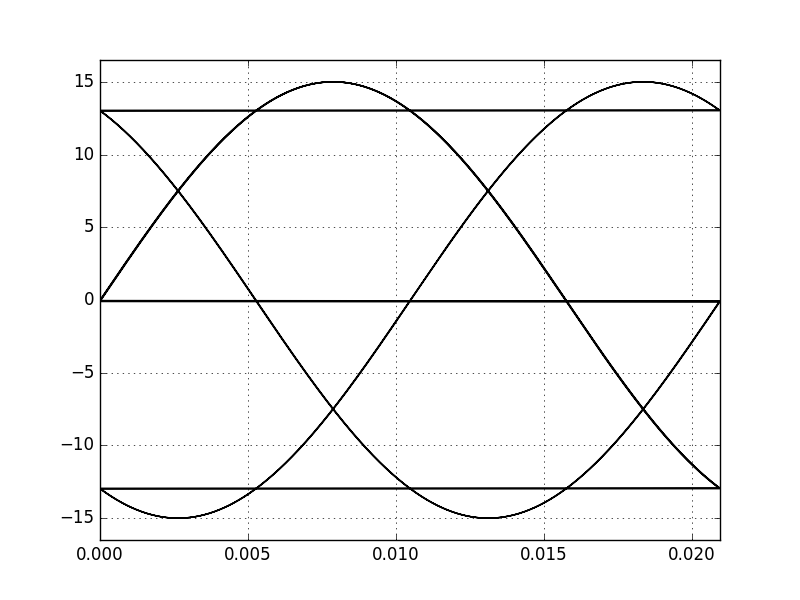
\includegraphics[width=0.8\textwidth]{freq-3-2-cross.png}
	\caption{Сигнал на экране осциллографа при $2\Tr=3\Ts$}
	\label{fig:cross}
\end{figure}

Глаз не будет видеть движение луча, если время послесвечения трубки -- время свечения экрана после прекращения возбуждения его электронным лучом -- больше перида развертки, и на экране будет видна сплошная линия. 

Заметим также, что во время обратного хода на модулятор трубки поступает отрицательное напряжение, запирающее луч, поэтому обратный ход луча на экране трубки не виден.

\subsection{Фигуры Лиссажу}

\begin{figure}[H]
	\centering
	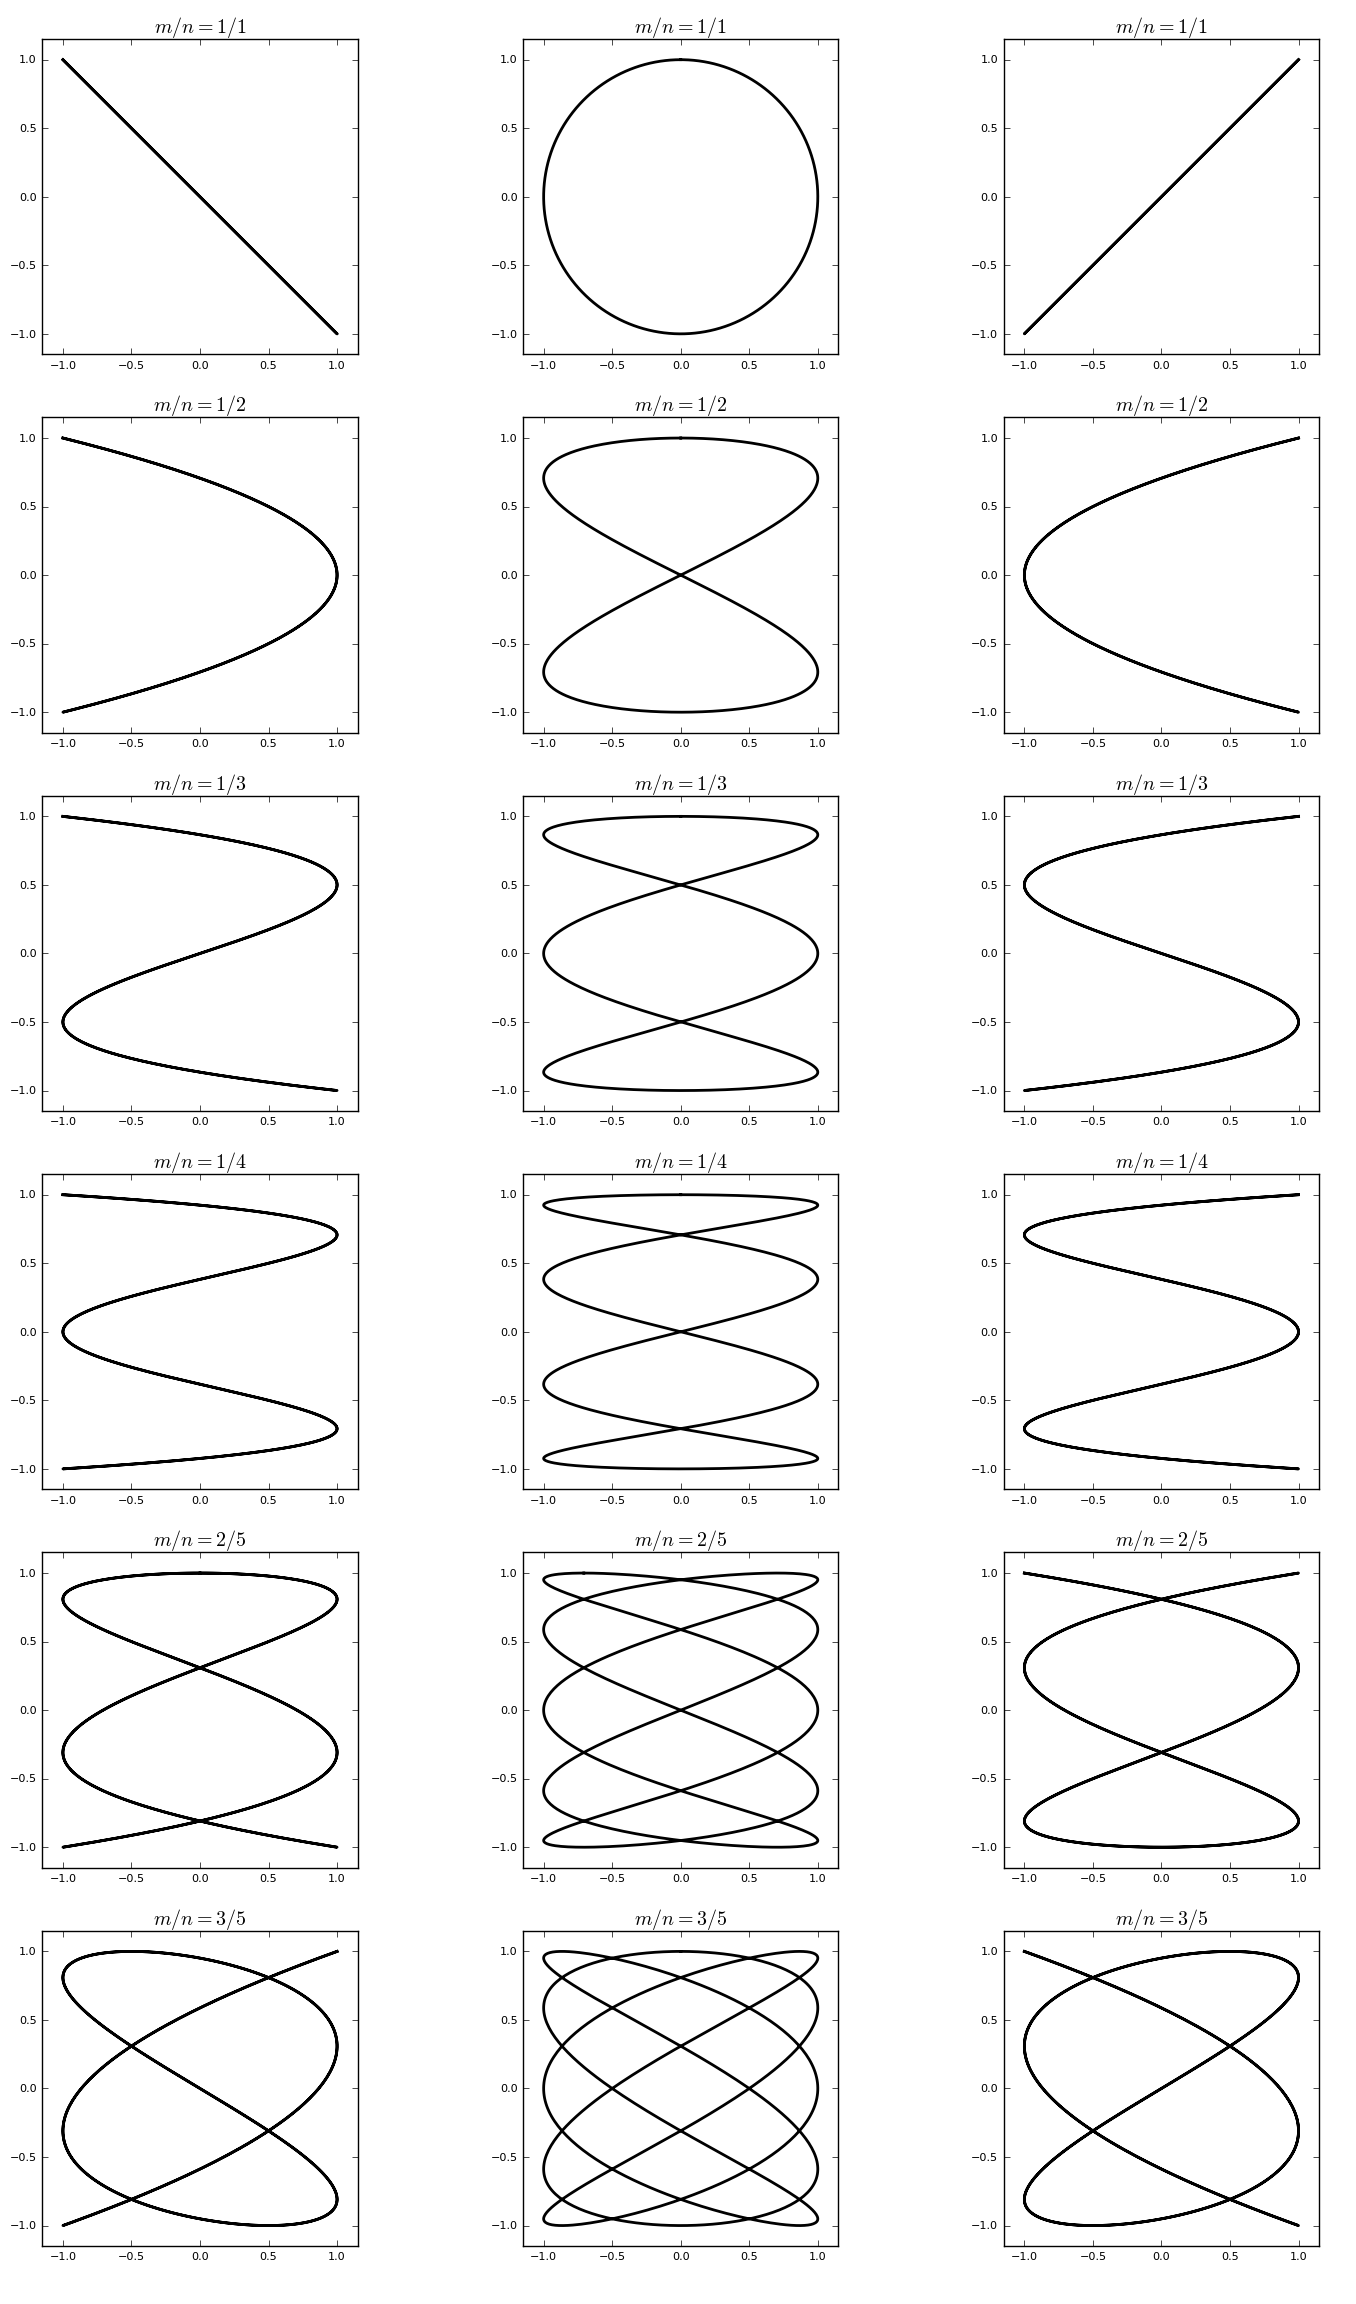
\includegraphics[width=0.8\textwidth]{lissajous3.png}
	\caption{Фигуры Лиссажу для $\frac{m}{n}=1;2;3;4;\frac{5}{2};\frac{5}{3}$}
	\label{fig:lissajous-1}
\end{figure}

\begin{figure}[H]
	\centering
	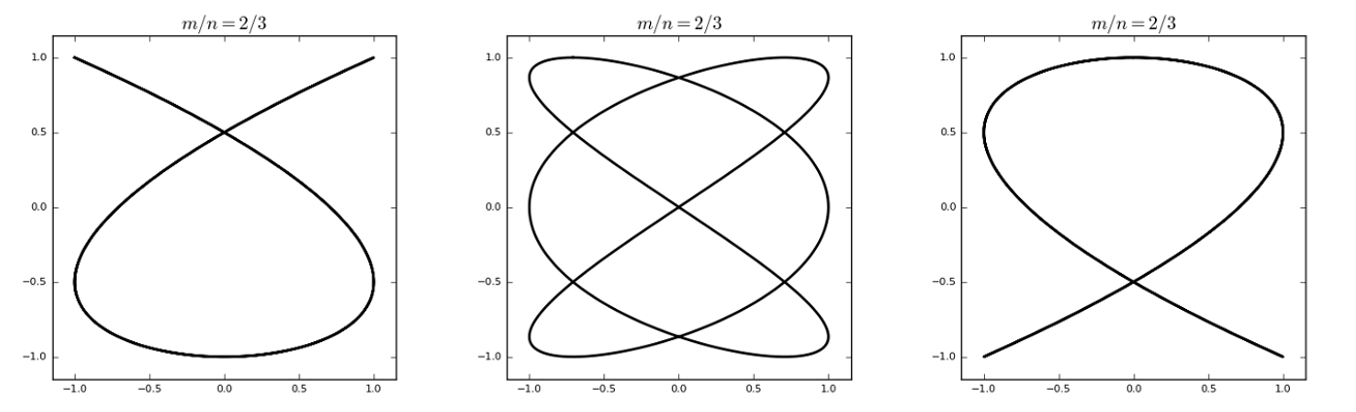
\includegraphics[width=0.85\textwidth]{lissajous2-3.png}
	\caption{Фигуры Лиссажу для $\frac{m}{n}=\frac{3}{2}$}
	\label{fig:lissajous-2}
\end{figure}

%%%%%%%%%%%%%%%%%%%%%%%%%%%%%%%%%%%%%%%%%%%%%%%%%%%%%%%%%%%%%
%%%%%%%%%%%%%%%%%%%%%%%%%%%%%%%%%%%%%%%%%%%%%%%%%%%%%%%%%%%%%


% \newpage
\section{Работа развертки осциллографа}
\subsection{Развертка сигнала}
\begin{figure}[H]
	\centering
	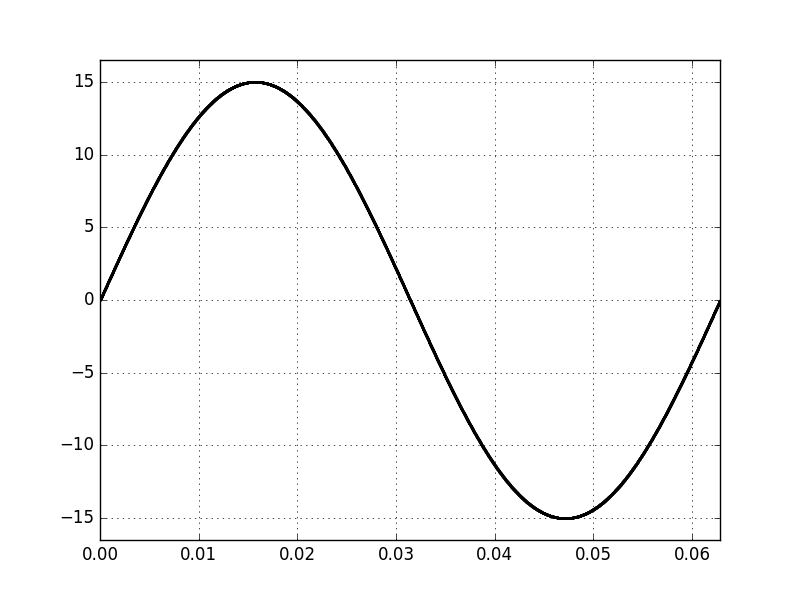
\includegraphics[width=0.85\textwidth]{freq-1-1.png}
	\caption{Развертка сигнала для $\frac{m}{n}=\frac{1}{1}$}
	\label{fig:freq-1-1}
\end{figure}

\begin{figure}[H]
	\centering
	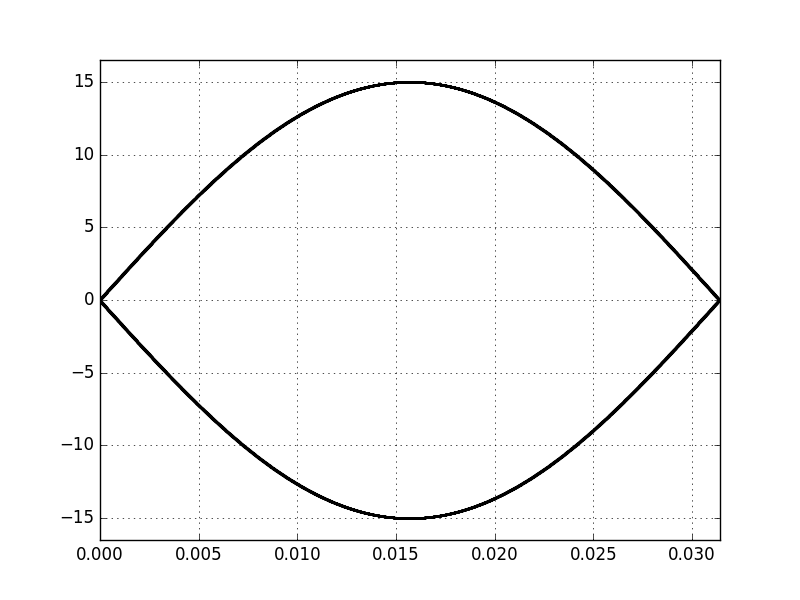
\includegraphics[width=0.85\textwidth]{freq-1-2.png}
	\caption{Развертка сигнала для $\frac{m}{n}=\frac{1}{2}$}
	\label{fig:freq-1-2}
\end{figure}

\begin{figure}[H]
	\centering
	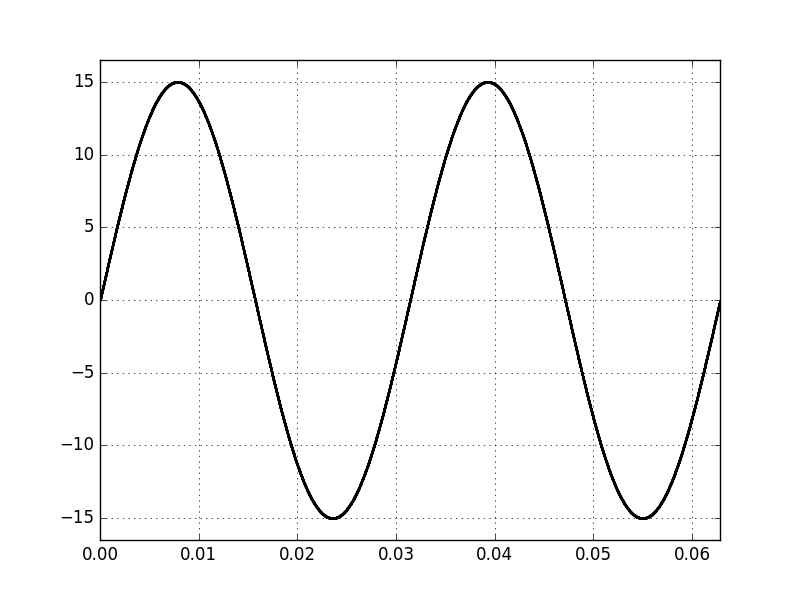
\includegraphics[width=0.85\textwidth]{freq-2-1.png}
	\caption{Развертка сигнала для $\frac{m}{n}=\frac{2}{1}$}
	\label{fig:freq-2-1}
\end{figure}

\begin{figure}[H]
	\centering
	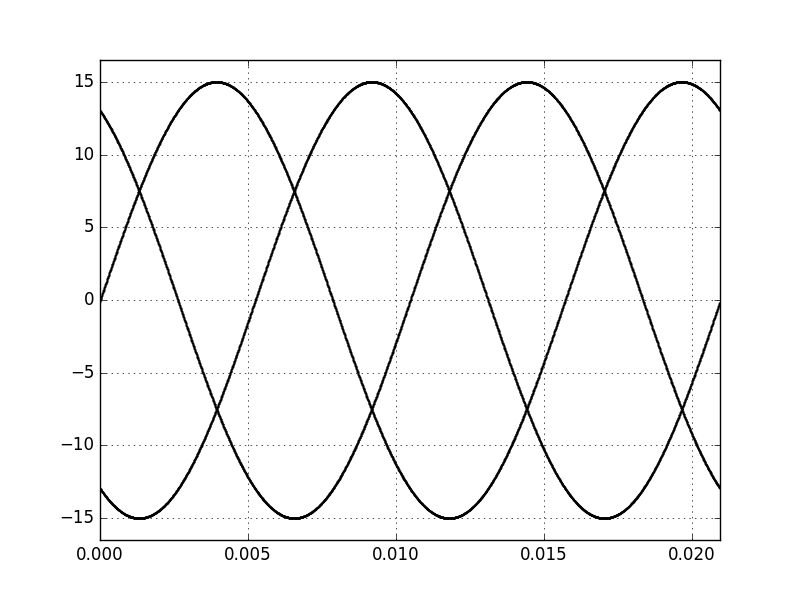
\includegraphics[width=0.85\textwidth]{freq-3-4.png}
	\caption{Развертка сигнала для $\frac{m}{n}=\frac{3}{4}$}
	\label{fig:freq-3-4}
\end{figure}

\begin{figure}[H]
	\centering
	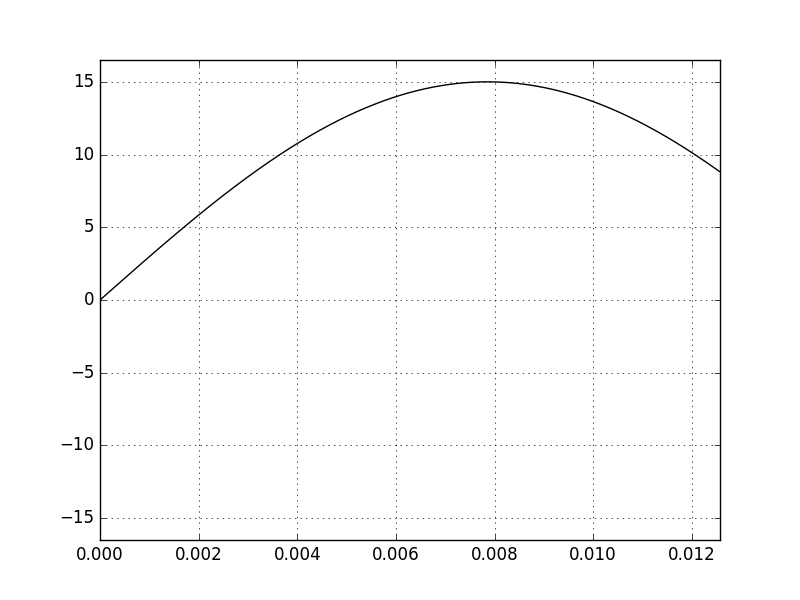
\includegraphics[width=0.85\textwidth]{freq-5-2.png}
	\caption{Развертка сигнала для $\frac{m}{n}=\frac{5}{2}$}
	\label{fig:freq-5-2}
\end{figure}

\subsection{Бегущая развертка}
\begin{figure}[H]
	\centering
	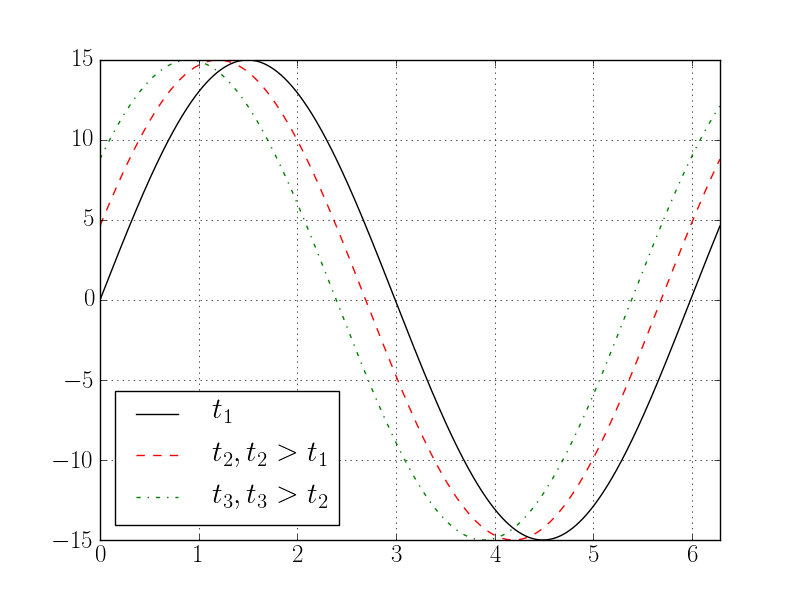
\includegraphics[width=0.85\textwidth]{freq-1-105.png}
	\caption{Бегущая развертка при $\frac{m}{n}=\frac{1}{1.05}$}
	\label{fig:freq-1-1.05}
\end{figure}

\begin{figure}[H]
	\centering
	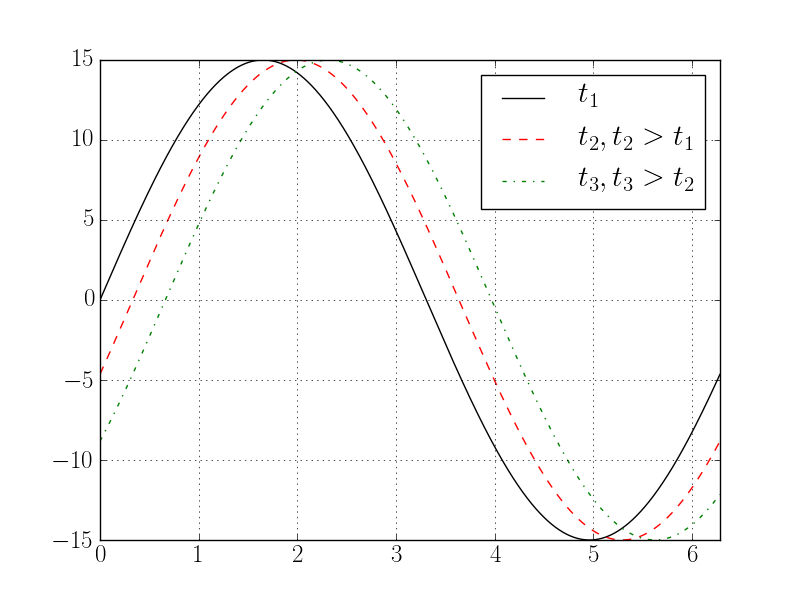
\includegraphics[width=0.85\textwidth]{freq-1-095.png}
	\caption{Бегущая развертка при $\frac{m}{n}=\frac{1}{0.95}$}
	\label{fig:freq-1-0.95}
\end{figure}


\section{Зоны синхронизации}
\begin{figure}[H]
	\centering
	% \includegraphics[]{}	
	\begin{tikzpicture}
	\hspace{-1cm}
		\draw[fill,yellow!60] 	
	% (1.5,0) --
	(0,0) --
	(3.0000,1.0000) --
	(4.5000,2.0000) --
	(6.0000,3.0000) --
	(6.7500,4.0000) --
	(7.5000,5.0000) --
	(9.0000,6.0000) --
	(9.7500,7.0000) --
	(10.5000,8.0000) --
	(12,\lft) --
	(\rft,\lft) --
	(\rft,-\lft) --
	(15.0000,-8.0000) --
	(13.5000,-7.0000) --
	(10.5000,-6.0000) --
	(9.0000,-5.0000) --
	(6.7500,-4.0000) --
	(5.2500,-3.0000) --
	(3.7500,-2.0000) --
	(2.2500,-1.0000) -- cycle;
			

\draw[step=.1cm , gray!20] (0,-\lft) grid (\rft ,\lft);
\draw[step=0.5cm , gray!50] (0,-\lft) grid (\rft ,\lft);
\draw[step=1cm , gray!80] (0,-\lft) grid (\rft ,\lft);


\draw[-{>[scale=1.0]}] (-0,0) -- (10*1.5 +1 ,0) node[anchor=north west] {\scalebox{1.5}{$A$}};
\draw[->] (0,-\lft) -- (0,\lft+1 ) node[anchor=east] {\scalebox{1.5}{$\frac{\nu_\text{с}-\nu_\text{р}}{\nu_\text{р}}$}};


\foreach \x in {1,2,3,4,5,6,7,8,9,10} {
	\draw (\x*\Xstep,0.05) -- (\x*\Xstep,-0.05);
	\draw (\x*\Xstep,0) node[anchor=north] {\scalebox{1.5}{$\x$}};
}

\foreach \y in {-0.3,-0.2,-0.1, 0, 0.1,0.2,0.3} {
	\draw (0.05,\y*\Ystep) -- (-0.05,\y*\Ystep);
	\draw (0,\y*\Ystep) node[anchor=east] {\scalebox{1.5}{$\y$}};
}

% \draw[blue] (15,0.5) node[anchor=east] {\scalebox{1.4}{Синхронизованная зона}};
% \draw[blue] (9.5,8.2) node[anchor=east] {\scalebox{1.4}{Несинхронизованная зона}};
% \draw[blue] (9.5,-8.3) node[anchor=east] {\scalebox{1.4}{Несинхронизованная зона}};
\input{experience/table.out}		
	\end{tikzpicture}
	\caption{Зоны синхронизации осциллографа. Диапазон частот -  20--200 Гц.}
	\label{fig:figure1}
\end{figure}

\newpage
\subsection{Вывод}


% \newpage
% \section*{Приложение 1. Графики зависимостей} % (fold)
% \label{sec:figures}

% section figures (end)

\end{document}
